\documentclass{beamer}
\usepackage[utf8]{inputenc}

\usetheme{Madrid}
\usecolortheme{default}
\usepackage{amsmath,amssymb,amsfonts,amsthm}
\usepackage{txfonts}
\usepackage{tkz-euclide}
\usepackage{listings}
\usepackage{adjustbox}
\usepackage{array}
\usepackage{tabularx}
\usepackage{gvv}
\usepackage{lmodern}
\usepackage{circuitikz}
\usepackage{tikz}
\usepackage{graphicx}

\setbeamertemplate{page number in head/foot}[totalframumber]

\usepackage{tcolorbox}
\tcbuselibrary{minted,breakable,xparse,skins}

\definecolor{bg}{gray}{0.95}
\lstset{
    language=C,
    basicstyle=\ttfamily\small,
    keywordstyle=\color{blue},
    stringstyle=\color{orange},
    commentstyle=\color{green!60!black},
    numbers=left,
    numberstyle=\tiny\color{gray},
    breaklines=true,
    showstringspaces=false,
}

%------------------------------------------------------------
\title{7.4.18}
\date{October 4,2025}
\author{EE25BTECH11011 - Navya Banavathu}

\begin{document}

\frame{\titlepage}

\begin{frame}{Question}
If the lines $3x-4y-7=0$ and $2x-3y-5=0$ are two diameters of a circle of area $49\pi$ square units, find the equation of the circle.

\begin{enumerate}
  \item $x^2+y^2+2x-2y-47=0$
  \item $x^2+y^2+2x-2y-62=0$
  \item $x^2+y^2-2x+2y-62=0$
  \item $x^2+y^2-2x+2y-47=0$
\end{enumerate}

\end{frame}

\begin{frame}{Solution}
Given two lines are,
\begin{align}
3x - 4y - 7 = 0 \\
2x - 3y - 5 = 0
\end{align}

Since the lines are diameters, the center lies on both:
\begin{align}
\mathbf{n}_1^T \mathbf{c} &= d_1, \\
\mathbf{n}_2^T \mathbf{c} &= d_2,
\end{align}
where
\begin{align}
\mathbf{n}_1 = \begin{bmatrix} 3 \\ -4 \end{bmatrix}, \quad d_1 = 7, \quad
\mathbf{n}_2 = \begin{bmatrix} 2 \\ -3 \end{bmatrix}, \quad d_2 = 5
\end{align}
\end{frame}

\begin{frame}{Solution}
In matrix form,
\begin{align}
\begin{bmatrix}
3 & -4 \\
2 & -3
\end{bmatrix}
\mathbf{c} =
\begin{bmatrix}
7 \\
5
\end{bmatrix}
\end{align}

The augmented matrix is
\begin{align}
\left[\begin{array}{cc|c}
3 & -4 & 7 \\
2 & -3 & 5
\end{array}\right]
\end{align}

Perform row operations to reduce it to RREF:
\begin{align}
\left[\begin{array}{cc|c}
3 & -4 & 7 \\
2 & -3 & 5
\end{array}\right]
&\;\xrightarrow{R_1 \rightarrow \frac{1}{3} R_1}\;
\left[\begin{array}{cc|c}
1 & -\frac{4}{3} & \frac{7}{3} \\
2 & -3 & 5
\end{array}\right]
\;\xrightarrow{R_2 \rightarrow R_2 - 2R_1}\;
\left[\begin{array}{cc|c}
1 & -\frac{4}{3} & \frac{7}{3} \\
0 & -\frac{1}{3} & \frac{1}{3}
\end{array}\right] \\
&\;\xrightarrow{R_2 \rightarrow -3 R_2}\;
\left[\begin{array}{cc|c}
1 & -\frac{4}{3} & \frac{7}{3} \\
0 & 1 & -1
\end{array}\right]
\;\xrightarrow{R_1 \rightarrow R_1 + \frac{4}{3} R_2}\;
\left[\begin{array}{cc|c}
1 & 0 & 1 \\
0 & 1 & -1
\end{array}\right]
\end{align}
\end{frame}

\begin{frame}{Solution}
Hence, the centre is
\begin{align}
\mathbf{c} = \begin{bmatrix} 1 \\ -1 \end{bmatrix}
\end{align}

The general conic form of a circle is
\begin{align}
g(\mathbf{x}) = \mathbf{x}^\top V \mathbf{x} + 2 \mathbf{u}^\top \mathbf{x} + f = 0, 
\end{align}

where $V = I$ for a circle. The centre satisfies
\begin{align}
V \mathbf{c} + \mathbf{u} = 0 \implies \mathbf{u} = -\mathbf{c}
= \begin{bmatrix} -1 \\ 1 \end{bmatrix}
\end{align}
\end{frame}

\begin{frame}{Solution}
Given the area $49\pi$, the radius squared is
\begin{align}
r^2 = 49.
\end{align}

Using the vector form relation for a circle:
\begin{align}
r^2 = \mathbf{u}^\top \mathbf{u} - f = 2 - f \implies f = -47.
\end{align}

Hence, the equation of the circle in vector form is
\begin{align}
\mathbf{x}^\top V \mathbf{x} + 2 \mathbf{u}^\top \mathbf{x} + f &= 0,
\end{align}

which in coordinates becomes
\begin{align}
x^2 + y^2 + 2(-1)x + 2(1)y - 47 &= 0, \\
\boxed{x^2 + y^2 - 2x + 2y - 47 = 0}.
\end{align}
\end{frame}
\begin{frame}[fragile]{ Code (C)}
\begin{block}{Part 1}
\begin{lstlisting}[language=C, basicstyle=\ttfamily\small, keywordstyle=\color{blue}, frame=single]
#include <stdio.h>
#include <math.h>

// Function to compute the circle equation parameters
void solve_circle(double *params) {
    double a1 = params[0];
    double b1 = params[1];
    double c1 = params[2];
    double a2 = params[3];
    double b2 = params[4];
    double c2 = params[5];
    double area = params[6];

    // Use direct numeric value of pi
    double pi = 3.141592653589793;
\end{lstlisting}
\end{block}
\end{frame}

\begin{frame}[fragile]{ Code (C)}
\begin{block}{Part 2}
\begin{lstlisting}[language=C, basicstyle=\ttfamily\small, keywordstyle=\color{blue}, frame=single]
 // Compute determinant to check if lines intersect
    double det = a1 * b2 - a2 * b1;
    if (fabs(det) < 1e-10) {
        printf("Lines are parallel or coincident. Cannot determine center.\n");
        return;
    }
    double rhs1 = -c1;
    double rhs2 = -c2;

    double h = (rhs1 * b2 - b1 * rhs2) / det;
    double k = (a1 * rhs2 - rhs1 * a2) / det;

    if (area <= 0) {
        printf("Area must be positive.\n");
        return;
    }
\end{lstlisting}
\end{block}
\end{frame}

\begin{frame}[fragile]{ Code (C)}
\begin{block}{Part 3}
\begin{lstlisting}[language=C, basicstyle=\ttfamily\small, keywordstyle=\color{blue}, frame=single]
 double r = sqrt(area / pi);

    // Compute circle coefficients
    double D = -2 * h;
    double E = -2 * k;
    double F = h * h + k * k - r * r;

    // Store results in params array
    params[7] = h;
    params[8] = k;
    params[9] = r;
    params[10] = D;
    params[11] = E;
    params[12] = F;
}
\end{lstlisting}
\end{block}
\end{frame}

\begin{frame}[fragile]{ Code (C)}
\begin{block}{Part 4}
\begin{lstlisting}[language=C, basicstyle=\ttfamily\small, keywordstyle=\color{blue}, frame=single]
int main() {
    double params[13];

    printf("Enter coefficients of first line (a1 b1 c1) for a1*x + b1*y + c1 = 0:\n");
    scanf("%lf %lf %lf", &params[0], &params[1], &params[2]);

    printf("Enter coefficients of second line (a2 b2 c2) for a2*x + b2*y + c2 = 0:\n");
    scanf("%lf %lf %lf", &params[3], &params[4], &params[5]);

    printf("Enter area of the circle (numeric):\n");
    scanf("%lf", &params[6]);


\end{lstlisting}
\end{block}
\end{frame}

\begin{frame}[fragile]{ Code (C)}
\begin{block}{Part 5}
\begin{lstlisting}[language=C, basicstyle=\ttfamily\small, keywordstyle=\color{blue}, frame=single]
 solve_circle(params);

    printf("\n--- Results ---\n");
    printf("Center (h, k): (%.3f, %.3f)\n", params[7], params[8]);
    printf("Radius: %.3f\n", params[9]);
    printf("Equation: x^2 + y^2 %+.3fx %+.3fy %+.3f = 0\n",
           params[10], params[11], params[12]);

    return 0;
}

\end{lstlisting}
\end{block}
\end{frame}

\begin{frame}[fragile]{Python Code:Import and Define points}
\begin{block}{Part 1}
\begin{lstlisting}[language=Python, basicstyle=\ttfamily\small, keywordstyle=\color{blue}, frame=single]
import ctypes
import os
import math
import numpy as np
import matplotlib.pyplot as plt

# Load the compiled C library
if os.name == "nt":   # Windows
    lib = ctypes.CDLL("./code13.dll")
else:
    lib = ctypes.CDLL("./code13.so")

# Define argument and return types for C function
lib.solve_circle.argtypes = [ctypes.POINTER(ctypes.c_double)]
lib.solve_circle.restype = None

\end{lstlisting}
\end{block}
\end{frame}


\begin{frame}[fragile]{Python Code}
\begin{block}{Part 2}
\begin{lstlisting}[language=Python, basicstyle=\ttfamily\small, keywordstyle=\color{blue}, frame=single]
# Input values (example from question)
# Lines: 3x - 4y - 7 = 0  and  2x - 3y - 5 = 0
# Area = 49π
a1, b1, c1 = 3, -4, -7
a2, b2, c2 = 2, -3, -5
area = 49 * math.pi

# Prepare array of doubles (13 elements)
params = (ctypes.c_double * 13)()
params[0] = a1
params[1] = b1
params[2] = c1
params[3] = a2
params[4] = b2
params[5] = c2
params[6] = area

\end{lstlisting}
\end{block}
\end{frame}


\begin{frame}[fragile]{Python Code}
\begin{block}{Part 3}
\begin{lstlisting}[language=Python, basicstyle=\ttfamily\small, keywordstyle=\color{blue}, frame=single]
# Call the C function
lib.solve_circle(params)

# Retrieve results
h, k, r, D, E, F = params[7], params[8], params[9], params[10], params[11], params[12]

# Print results
print("\n--- Circle Parameters ---")
print(f"Center (h, k): ({h:.3f}, {k:.3f})")
print(f"Radius: {r:.3f}")
print(f"Equation: x^2 + y^2 {D:+.3f}x {E:+.3f}y {F:+.3f} = 0")
\end{lstlisting}
\end{block}
\end{frame}


\begin{frame}[fragile]{Python Code: Plotting}
\begin{block}{Part 4}
\begin{lstlisting}[language=Python, basicstyle=\ttfamily\small, keywordstyle=\color{blue}, frame=single]
# Plot circle and diameter lines
theta = np.linspace(0, 2 * np.pi, 400)
x_circle = h + r * np.cos(theta)
y_circle = k + r * np.sin(theta)

# Lines
x_vals = np.linspace(-10, 10, 300)
y1 = (a1 * x_vals + c1) / (-b1)
y2 = (a2 * x_vals + c2) / (-b2)

plt.figure(figsize=(6, 6))
plt.plot(x_circle, y_circle, 'b', label='Circle')
plt.plot(x_vals, y1, 'r--', label=f'{a1}x {b1:+}y {c1:+} = 0')
plt.plot(x_vals, y2, 'g--', label=f'{a2}x {b2:+}y {c2:+} = 0')
\end{lstlisting}
\end{block}
\end{frame}

\begin{frame}[fragile]{Python Code: Plotting}
\begin{block}{Part 5}
\begin{lstlisting}[language=Python, basicstyle=\ttfamily\small, keywordstyle=\color{blue}, frame=single]
plt.scatter(h, k, color='black', s=50, label='Center (1,-1)')
plt.text(h, k, '  (1, -1)', fontsize=10, color='black', va='center', ha='left')
plt.title("Circle with Given Diameter Lines")
plt.xlabel("x-axis")
plt.ylabel("y-axis")
plt.grid(True)
plt.legend()
plt.axis('equal')

# Save figure as fig13.png
plt.savefig("fig13.png", dpi=300)

# Show the figure
plt.show()
\end{lstlisting}
\end{block}
\end{frame}

\begin{frame}{Graphical Representation}
    \begin{figure}
        \centering
        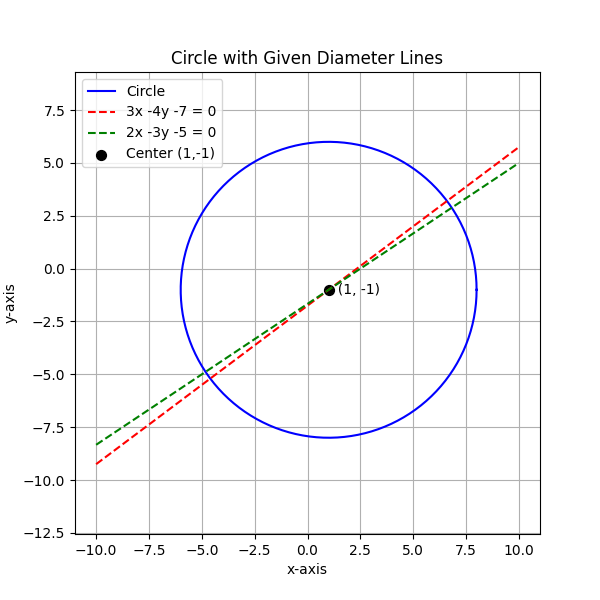
\includegraphics[width=0.6\columnwidth]{../beamer/figs/fig13.png}
    \end{figure}
\end{frame}

\end{document}

